\documentclass[a3paper, landscape]{eskdgraph}

\usepackage{env}

% Код
\ESKDletter{}{К}{Р}
\def \gpiDocTypeNum {90}
\def \gpiDocVer {00}
\def \gpiCode {\ESKDtheLetterI\ESKDtheLetterII\ESKDtheLetterIII.\gpiStudentGroupName\gpiStudentGroupNum.\gpiStudentCard-0\gpiDocNum~\gpiDocTypeNum~\gpiDocVer}

\def \gpiDocTopic {СХЕМА ПРОГРАММЫ}

% Графа 1 (наименование изделия/документа)
\ESKDcolumnI {\ESKDfontIII \gpiTopic \\ \gpiDocTopic}

% Графа 2 (обозначение документа)
\ESKDsignature {\gpiCode}

% Графа 9 (наименование или различительный индекс предприятия) задает команда
\ESKDcolumnIX {\gpiDepartment}

% Графа 11 (фамилии лиц, подписывающих документ) задают команды
\ESKDcolumnXIfI {\gpiStudentSurname}
\ESKDcolumnXIfII {\gpiTeacherSurname}
\ESKDcolumnXIfV {\gpiTeacherSurname}

\begin{document}
    \hspace{0pt}
    \begin{figure}[!h]
        \centering
        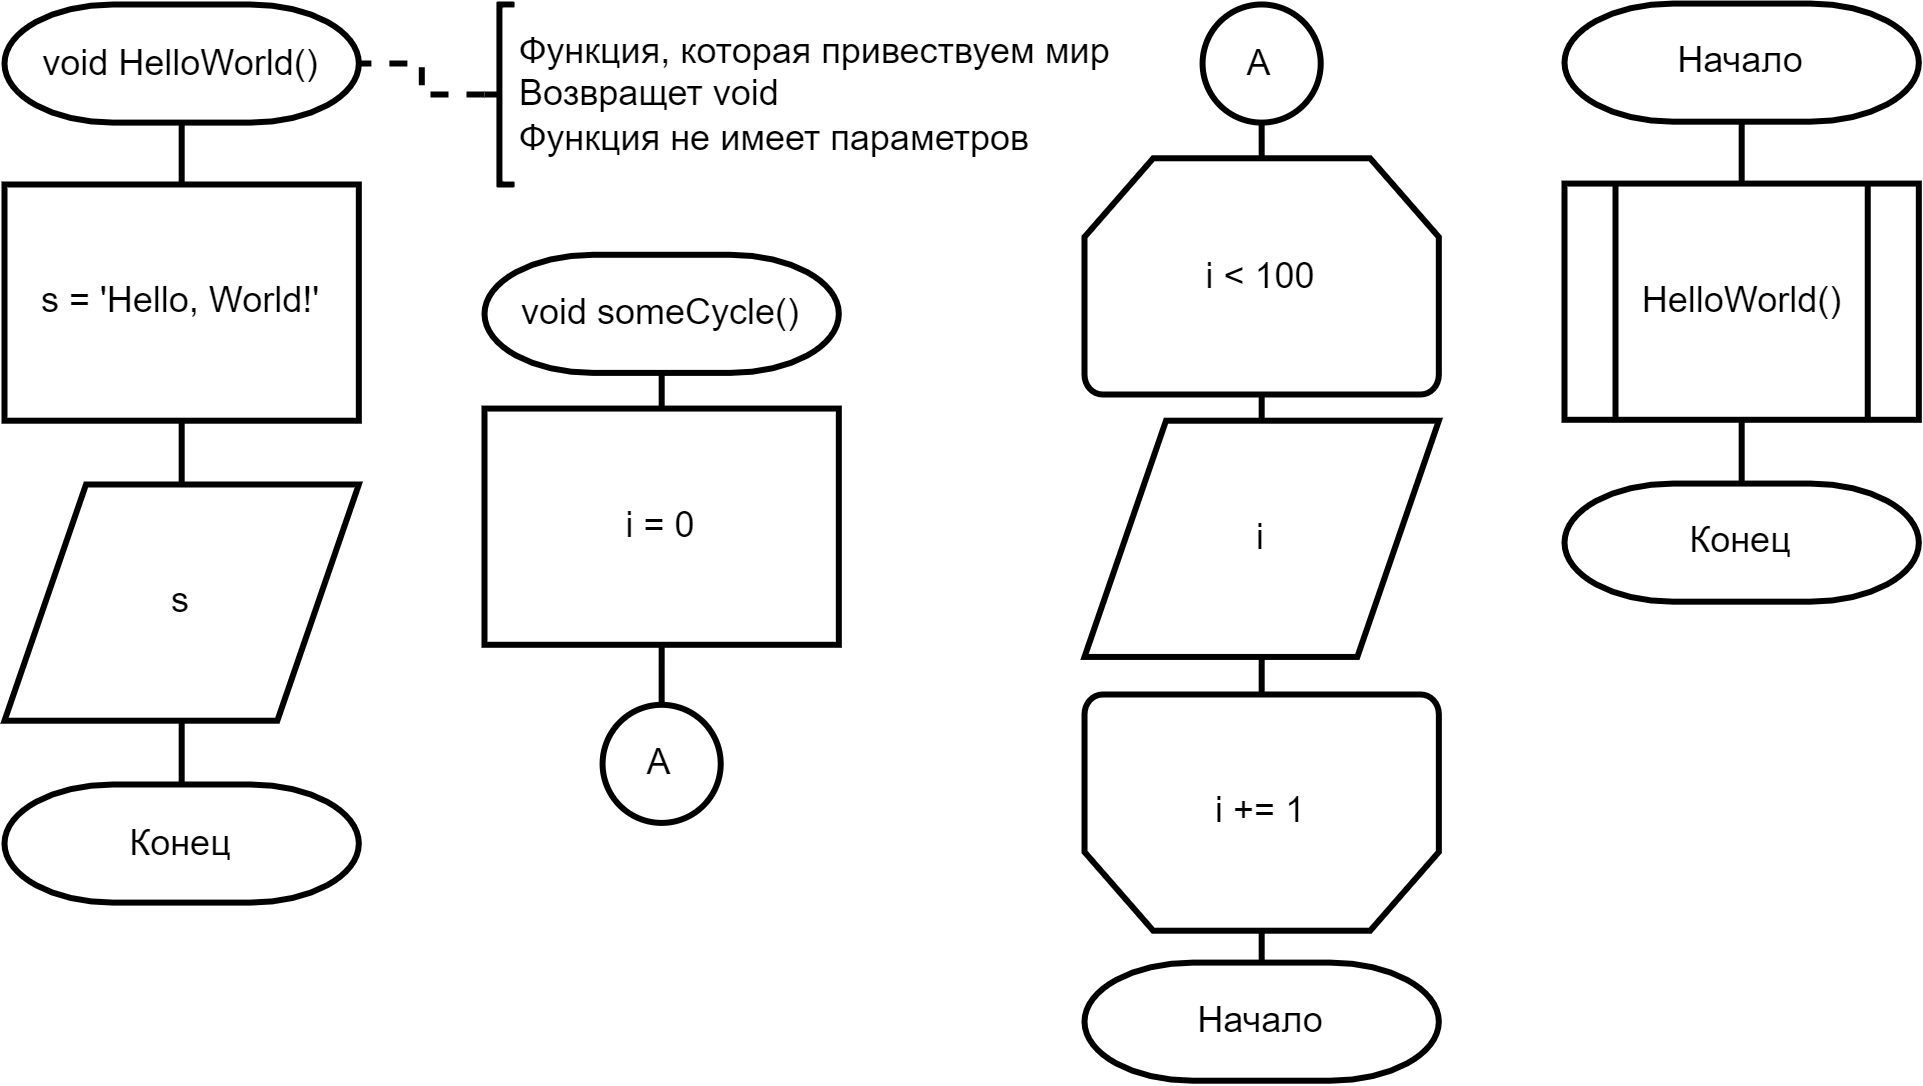
\includegraphics[]
            {_assets/Flowcharts.png}
    \end{figure}
\end{document}
